\section{Arquitetura}

Nessa seção do capítulo, apresenta-se a arquitetura da aplicação, que define como os componentes do sistema interagem entre si e com o usuário.

\subsection{Definições da arquitetura}

O sistema foi estruturado com base no modelo cliente-servidor, no qual o front-end e o back-end operam como aplicações independentes que se comunicam por meio de requisições HTTP, seguindo a arquitetura RESTful.

O back-end é responsável pelo processamento da lógica de negócios e pela persistência dos dados, enquanto o front-end realiza a apresentação e interação com o usuário. Essa separação garante maior modularidade e facilita a manutenção da aplicação, cujo domínio é um ambiente de \textit{coworking} para salões de beleza.

A arquitetura do sistema adota um padrão baseado no Model-View-Controller (MVC) de forma adaptada, aproximando-se de uma arquitetura em camadas. Cada camada possui uma responsabilidade bem definida, conforme descrito a seguir:

\begin{itemize}
  \item \textbf{Controller:} Responsável por receber e tratar as requisições provenientes do cliente (front-end), encaminhando-as para a camada de serviço correspondente. Esta camada lida diretamente com aspectos de infraestrutura externa,  como servidores de borda ou gateways de entrada da aplicação, servindo como ponto inicial de processamento das solicitações.
  \item \textbf{Service:} Centraliza a lógica de negócio da aplicação. É responsável por processar as regras do domínio e pode tanto consumir outras funções de serviço quanto interagir com a camada de persistência.
  \item \textbf{Repository:} Trata das operações relacionadas à persistência de dados. Atua como uma interface entre os serviços e os mecanismos de armazenamento, como bancos de dados relacionais ou caches, promovendo o desacoplamento da lógica de negócio em relação à camada de dados.
\end{itemize}

\subsection{Diagrama da arquitetura}

Esta subseção apresenta dois diagramas que representam a arquitetura do sistema desenvolvido: o diagrama de componentes e o diagrama de implantação. Esses diagramas auxiliam na visualização do relacionamento entre as partes da aplicação, bem como a sua distribuição nos ambientes computacionais.

\subsubsection{Diagrama de componentes}

O diagrama de componentes representa a organização lógica dos principais módulos da aplicação, evidenciando as dependências e as formas de comunicação entre eles. Ele demonstra como os componentes interagem por meio de interfaces — que definem contratos de uso — e implementações — que oferecem as funcionalidades esperadas.

Esse tipo de diagrama é útil para visualizar a estrutura modular da aplicação, facilitando o entendimento da separação de responsabilidades e da reutilização de código, além de apoiar decisões relacionadas à manutenção e evolução do sistema.

\begin{figure}[htb]
  \centering
  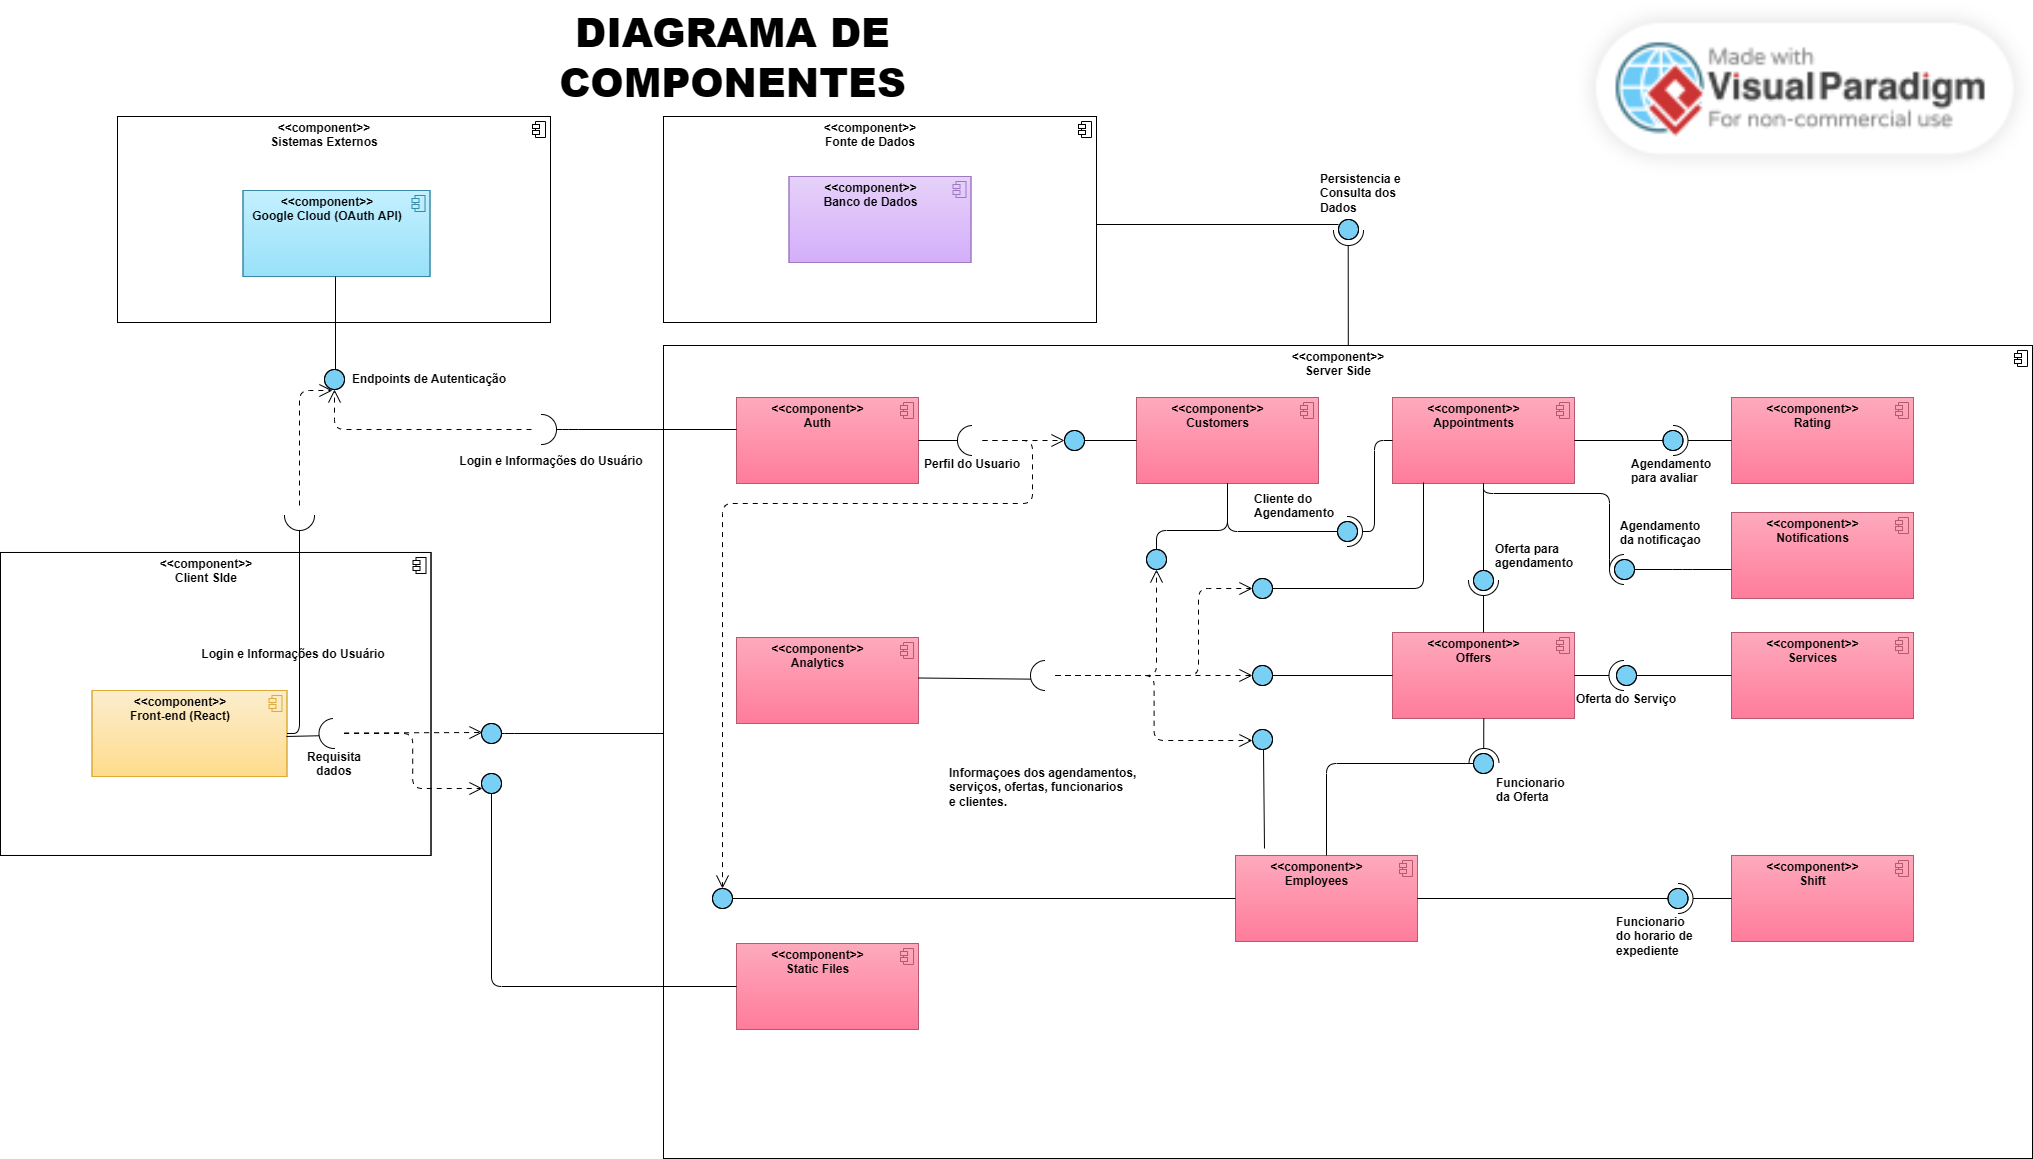
\includegraphics[width=\textwidth]{cap04-desenvolvimento/images/4-3-2-1-diagrama-componentes}
  \caption{Diagrama de componente da aplicação}
  \label{fig:diagrama-componente}
\end{figure}


No diagrama de componentes proposto, a aplicação é composta por diversos módulos que representam funcionalidades distintas e organizadas de forma modular. Esses componentes são responsáveis por encapsular regras de negócio e oferecer interfaces bem definidas para comunicação entre si. A seguir, são descritos os principais módulos do sistema:

\begin{itemize}
  \item \textbf{Auth}: Componente responsável pela autenticação de usuários e integração com serviços externos, como o Google OAuth. Garante um processo facilitado de login para os usuários e autenticação no acesso das funcionalidades protegidas da aplicação.

  \item \textbf{Analytics}: Responsável por gerar relatórios e fornecer estatísticas baseadas nas informações do sistema. Auxilia principalmente no acompanhamento de desempenho da plataforma por parte dos gerentes do salão.

  \item \textbf{Appointments}: Gerencia os agendamentos realizados pelos clientes. Engloba tanto a criação, listagem e atualização dos agendamentos quanto a associação com os serviços ofertados.

  \item \textbf{Customers}: Controla os dados relacionados aos clientes da plataforma. Permite o cadastro, consulta e edição de informações do perfil dos usuários.

  \item \textbf{Employees}: Administra os dados dos profissionais que prestam serviços na aplicação, incluindo informações cadastrais, disponibilidade e associação a serviços específicos.

  \item \textbf{Notifications}: Responsável por enviar notificações aos usuários, como lembretes, confirmações de agendamento e atualizações importantes. Pode incluir o envio por e-mail ou outros canais.

  \item \textbf{Offers}: Define a relação entre profissionais e os serviços que eles oferecem. Cada oferta especifica o tempo estimado e o valor cobrado por um funcionário para realizar determinado serviço. Esse componente é fundamental para a composição de um agendamento, pois determina quais combinações de profissional e serviço estão disponíveis.

  \item \textbf{Services}: Representa os serviços oferecidos pela empresa, armazenando informações descritivas como nome e descrição. Este módulo não define valores ou tempos de execução, pois esses dados são especificados nas ofertas individuais de cada profissional (por meio do módulo \textit{Offers}).

  \item \textbf{Shift}: Trata do controle de turnos de trabalho dos funcionários, possibilitando a definição de horários disponíveis para realização dos agendamentos.

  \item \textbf{Rating}: Permite que os clientes avaliem os serviços e os profissionais após os atendimentos, promovendo um sistema de feedback contínuo.
  
  \item \textbf{Role e Permissions}: Implementa o controle de acesso baseado em papéis, estabelecendo diferentes níveis de permissão conforme o tipo de usuário (cliente, funcionário, administrador, etc.).

  \item \textbf{Static Files (Front-end)}: Componente responsável por servir os arquivos estáticos da interface do usuário, gerados após o processo de \textit{build} do projeto front-end (em React). Inclui arquivos HTML, CSS e JavaScript que são entregues ao navegador do usuário final via servidor NGINX.
\end{itemize}

\subsubsection{Diagrama de Implantação}

O diagrama de implantação mostra como os componentes do sistema estão distribuídos em termos de infraestrutura, seja em servidores físicos ou ambientes virtuais. Ele ajuda a entender onde cada parte da aplicação está rodando, como os serviços se conectam entre si e quais recursos são necessários para que tudo funcione bem em produção.

Esse tipo de representação é especialmente útil para quem for implantar ou manter o sistema, pois facilita a visualização de elementos como servidores, banco de dados, gateways de rede, e outras dependências da aplicação. Além disso, o diagrama contribui para o planejamento de permissões, acessos e políticas de segurança que precisam ser configuradas na infraestrutura.

\begin{figure}[htb]
  \centering
  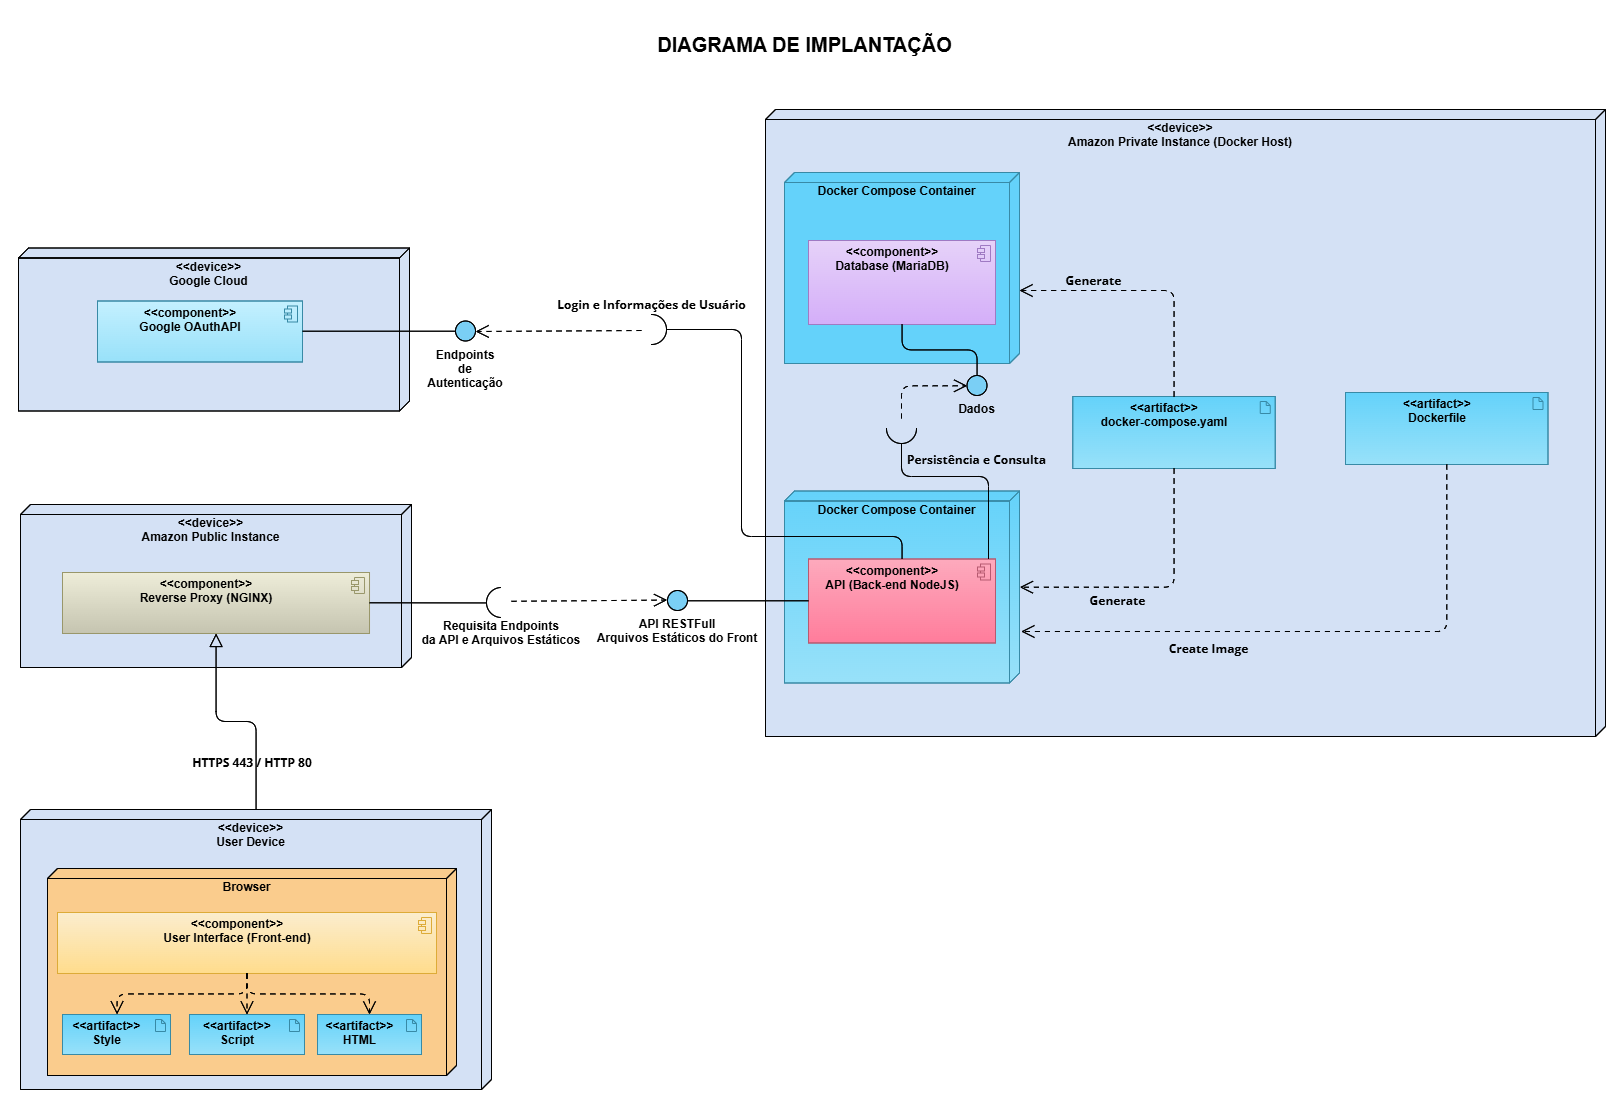
\includegraphics[width=\textwidth]{cap04-desenvolvimento/images/4-3-2-2-diagrama-implantacao}
  \caption{Diagrama de implantação da aplicação}
  \label{fig:diagrama-implantacao}
\end{figure}

O diagrama acima é composto pelos seguintes componentes:
\begin{itemize}
  \item \textbf{\textit{User Device:}} No diagrama proposto, por se tratar de uma aplicação web, o dispositivo do usuário será responsável por executar a aplicação \textit{client-side}, que interpreta através do navegador os arquivos CSS, JavaScript e HTML gerados no empacotamento ou \textit{build} do projeto feito com a biblioteca React. Ademais, esse \textit{device} é composto por alguns artefatos importantes que são obtidos pelo navegador por meio de uma requisição ao \textit{Proxy Reverso}: CSS (style), JavaScript (script) e HTML.

  \item \textbf{\textit{Amazon Public Instance (Device):}} A \textit{Amazon Public Instance} é uma instância EC2 que possui um IP público, o que permite que ela seja acessada diretamente pelo usuário ou resolvida por DNS. Por esse motivo, nela são executados apenas os componentes que devem estar disponíveis publicamente ao cliente final:
    \begin{itemize}
      \item \textit{Componente NGINX}: Serviço que atua como \textit{Proxy Reverso} para a aplicação que está sendo executada em uma instância privada na arquitetura proposta. Para viabilizar conexões HTTPS, o NGINX utiliza certificados digitais emitidos gratuitamente pelo serviço Let's Encrypt, por meio da ferramenta Certbot, que automatiza todo o processo de emissão e renovação dos certificados~\cite{LetsEncryptWithCertbot}. Este serviço é instalado como um \textbf{artefato} adicional no ambiente da instância pública, sendo integrado ao próprio ciclo de configuração e inicialização do NGINX.
    \end{itemize}

  \item \textbf{\textit{Amazon Private Instance (Device):}} Por outro lado, a \textit{Amazon Private Instance} é composta por uma instância EC2 com restrições de rede, o que significa que seu acesso é limitado à rede interna e não possui IP público. Nessa instância, componentes da arquitetura que não precisam estar disponíveis de forma pública são o caso de uso perfeito, uma vez que garante maior segurança e isolamento dos aspectos internos da aplicação. Em seu interior, ela é composta pelos seguintes componentes:
    \begin{itemize}
      \item \textit{API (Back-end em NodeJS)}: Principal serviço da aplicação, sendo o responsável por se prover os "endpoints" que fornecem os dados e arquivos estáticos para o \textit{front-end} através de uma \textit{API RestFull}, se comunicando com o banco de dados, um componente que é executado no mesmo device.
      \item \textit{Banco de Dados (SGBD MariaDB)}: Serviço de \textit{SGBD} que provê os dados para o \textit{back-end} da aplicação, o que possibilita a persistência e consulta de forma eficiente. Para garantir a persistência dos dados gerenciados pelo MariaDB, o contêiner utiliza volumes Docker montados na instância EC2 privada. Isso assegura que os dados não sejam perdidos em reinicializações do contêiner.
    \end{itemize}
  Além dos serviços em execução, a instância privada também contém os seguintes artefatos essenciais para o empacotamento e execução dos serviços via contêineres Docker:
    \begin{itemize}
      \item \textit{Dockerfile}: Esse artefato descreve as instruções necessárias para criar a imagem Docker da aplicação \textit{back-end}, especificando o ambiente base (como a imagem do Node.js), os arquivos a serem copiados, dependências a serem instaladas e os comandos de inicialização da aplicação.

      \item \textit{docker-compose.yaml}: Esse arquivo é utilizado como ferramenta de orquestração para os serviços Docker da aplicação. Ele define a configuração dos contêineres da aplicação, como o contêiner da API e o do banco de dados, bem como as variáveis de ambiente, volumes, redes e dependências entre os serviços. É a partir deste artefato que os contêineres são gerados e executados de forma integrada.
    \end{itemize}

  \item \textbf{\textit{Google Cloud (Device):}} Localizada na nuvem pública da Google (\textit{Google Cloud}), essa API é utilizada pelo back-end da aplicação para realizar a autenticação de usuários através do protocolo OAuth 2.0 \cite{GoogleOAuth}. Esse processo ocorre quando o usuário opta por fazer login com sua conta Google. Nesse cenário, a aplicação redireciona o usuário para a tela de autenticação da Google, e após a confirmação, a API recebe um \textit{token} de acesso que é utilizado para obter as informações do usuário autenticado. Esse fluxo garante uma autenticação segura, delegando a responsabilidade da validação de identidade à Google.
\end{itemize}

O fluxo de execução típico da aplicação baseado no diagrama de implantação acima segue os seguintes passos:
\begin{enumerate}
  \item O usuário acessa a aplicação pelo navegador, requisitando os arquivos HTML/CSS/JS ao servidor NGINX.
  \item O NGINX, atuando como proxy reverso, redireciona essas requisições para o serviço de back-end na instância privada.
  \item A API processa a requisição, acessa o banco de dados quando necessário e retorna os dados.
  \item Em caso de autenticação via Google, a API redireciona o usuário para o serviço Google OAuth, que retorna um token de acesso após o login.
  \item Esse token é utilizado pela API para obter os dados do usuário autenticado e estabelecer uma sessão.
\end{enumerate}

Além da organização dos componentes do diagrama, a arquitetura também prioriza a segurança da comunicação e do acesso. O tráfego entre o navegador do usuário e a instância pública é realizado por meio do protocolo HTTPS, o que garante a confidencialidade e a integridade dos dados transmitidos. Para isso, foi utilizado o serviço gratuito de certificação digital Let's Encrypt em conjunto com a ferramenta Certbot, que automatiza a emissão, renovação e instalação dos certificados TLS no servidor NGINX.

Internamente, a comunicação entre o NGINX e os serviços da instância privada ocorre por meio de regras específicas de segurança definidas na VPC, utilizando mecanismos como \textit{Security Groups} e \textit{Route Tables}. Isso reduz significativamente a superfície de ataque da aplicação e assegura uma camada adicional de proteção para os aspectos internos.

\subsubsection{Diagrama de Referência na AWS}

Com o objetivo de fornecer uma visão mais aprofundada da infraestrutura da aplicação na nuvem, o diagrama apresenta a disposição dos principais componentes implantados na arquitetura da Amazon Web Services (AWS). 

Este diagrama ilustra elementos de infraestrutura fundamentais como sub-redes públicas e privadas, resolução de DNS, Virtual Private Cloud (VPC), Bastion Server, NAT Gateway, Internet Gateway, banco de dados, entre outros recursos. A representação facilita a compreensão técnica da topologia de rede e da distribuição dos serviços, evidenciando como a aplicação foi projetada para atender requisitos de segurança, escalabilidade e disponibilidade no ambiente da AWS. A seguir, descreve-se brevemente cada elemento presente no diagrama.

\begin{figure}[htb]
  \centering
  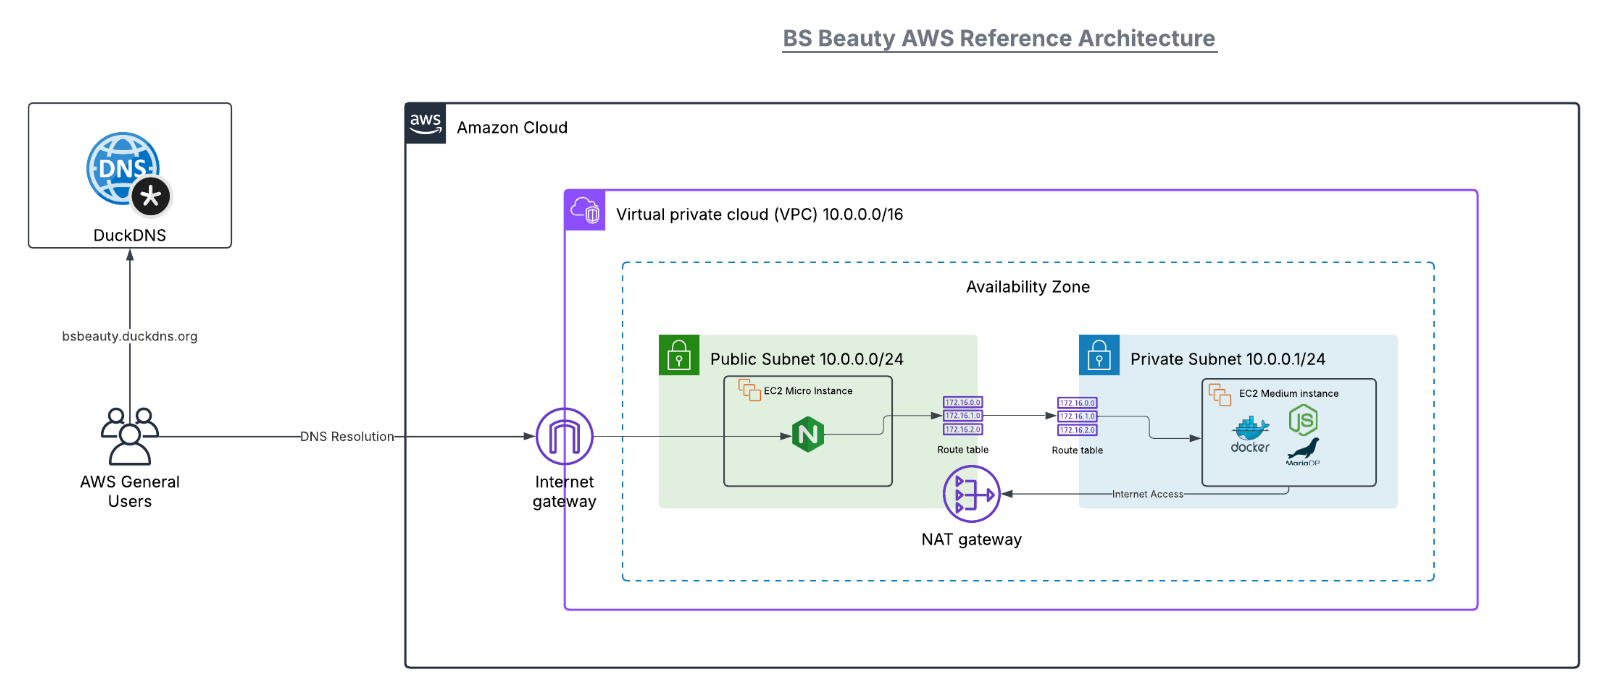
\includegraphics[width=\textwidth]{cap04-desenvolvimento/images/4-3-2-3-diagrama-geral}
  \caption{Diagrama Geral da Arquitetura}
  \label{fig:diagrama-geral}
\end{figure}

\begin{itemize}
  \item \textbf{VPC (Virtual Private Cloud):} A aplicação opera dentro de uma VPC personalizada com o bloco CIDR \texttt{10.0.0.0/16}, que abriga duas sub-redes: uma pública e outra privada, seguindo o princípio de segmentação de rede recomendado pela própria AWS~\cite{AWSBestPractices}.

  \item \textbf{Sub-rede pública (10.0.0.0/24):} Contém uma instância EC2 de pequeno porte (\texttt{t2.micro}) que executa o serviço NGINX. Esse servidor atua como proxy reverso, roteando as requisições provenientes da internet para os serviços internos hospedados em uma sub-rede privada.

  \item \textbf{Sub-rede privada (10.0.0.1/24):} Hospeda uma instância EC2 de médio porte (\texttt{t2.medium}), na qual são executados os contêineres da aplicação via Docker Compose, incluindo o serviço de back-end (Node.js) e o banco de dados relacional MariaDB.

  \item \textbf{NAT Gateway:} Permite que os recursos da sub-rede privada (como a instância EC2 que executa os contêineres) realizem atualizações e acessos à internet de forma segura, sem que sejam diretamente acessíveis externamente.

  \item \textbf{Internet Gateway:} Responsável por permitir o tráfego de entrada e saída entre a VPC e a internet pública. Está associado à sub-rede pública e NAT Gateway, permitindo que o NGINX receba requisições externas e o NAT receba um IP.

  \item \textbf{DuckDNS:} Utilizado como serviço de DNS dinâmico gratuito, permitindo que a aplicação seja acessada por um domínio estável (\texttt{bsbeauty.duckdns.org}), mesmo que o endereço IP público da instância EC2 varie. A resolução de nome é feita de forma transparente para o usuário final, facilitando o acesso à aplicação.

  \item \textbf{Usuários externos (AWS General Users):} Representam os clientes que acessam a aplicação via navegador. O tráfego HTTP/HTTPS chega inicialmente ao serviço NGINX na sub-rede pública, que encaminha as requisições para a instância privada onde os serviços da aplicação estão efetivamente em execução.
\end{itemize}

Essa separação entre sub-rede pública e privada visa seguir boas práticas de segurança e isolamento de ambiente, recomendadas tanto pela documentação oficial da AWS quanto por autores renomados da área de arquitetura de software em nuvem, como em \cite{AWSBestPractices}. Ao manter os serviços internos em uma sub-rede privada, reduz-se a superfície de ataque da aplicação e melhora a resistência contra acessos não autorizados.

Além disso, a utilização do DuckDNS simplifica a exposição da aplicação para o ambiente externo sem a necessidade de configurar manualmente um serviço de DNS ou pagar por domínios personalizados, o que se alinha aos objetivos de custo deste projeto.